%%% Econ712: Macroeconomics I
%%% Fall 2020
%%% Danny Edgel
%%%
% Due on Canvas Thursday December 3rd, 11:59pm Central Time
%%%

%%%
%							PREAMBLE
%%%

\documentclass{article}

%%% declare packages
\usepackage{amsmath}
\usepackage{amssymb}
\usepackage{array}
\usepackage{bm}
\usepackage{changepage}
\usepackage{centernot}
\usepackage{graphicx}
\usepackage[shortlabels]{enumitem}
\usepackage{fancyhdr}
	\fancyhf{} % sets both header and footer to nothing
	\renewcommand{\headrulewidth}{0pt}
    \rfoot{Edgel, \thepage}
    \pagestyle{fancy}
	
%%% define shortcuts for set notation
\newcommand{\N}{\mathbb{N}}
\newcommand{\Z}{\mathbb{Z}}
\newcommand{\R}{\mathbb{R}}
\newcommand{\Q}{\mathbb{Q}}
\newcommand{\lmt}{\underset{x\rightarrow\infty}{\text{lim }}}
\newcommand{\neglmt}{\underset{x\rightarrow-\infty}{\text{lim }}}
\newcommand{\zerolmt}{\underset{x\rightarrow 0}{\text{lim }}}
\newcommand{\loge}[1]{\text{ln}\left(#1\right)}
\newcommand{\usmax}[1]{\underset{#1}{\text{max }}}
\newcommand{\Mt}{M_{t+1}^t}
\newcommand{\vhat}{\hat{v}}
\newcommand{\olp}{\overline{p}}
\renewcommand{\L}{\mathcal{L}}
\newcommand{\olq}{\overline{q}}
\newcommand{\zinf}{_{t=0}^\infty}
\newcommand{\aneg}{A^{-1}}
\newcommand{\sneg}{s^{-1}}
\newcommand{\olk}{\overline{k}}
\newcommand{\olc}{\overline{c}}
\newcommand{\olr}{\overline{r}}
\newcommand{\olpi}{\overline{\pi}}
\newcommand{\Aneg}{A^{-1}}
\renewcommand{\sneg}{s^{-1}}
\newcommand{\dc}[1]{\Delta c_{#1}}

\newcommand{\E}[1]{\mathbb{E}\left[#1\right]} % expected value
\newcommand{\Et}[1]{\mathbb{E}_t\left[#1\right]}

%%% define column vector command (from Michael Nattinger)
\newcount\colveccount
\newcommand*\colvec[1]{
        \global\colveccount#1
        \begin{pmatrix}
        \colvecnext
}
\def\colvecnext#1{
        #1
        \global\advance\colveccount-1
        \ifnum\colveccount>0
                \\
                \expandafter\colvecnext
        \else
                \end{pmatrix}
        \fi
}

%%% define function for drawing matrix augmentation lines
\newcommand\aug{\fboxsep=-\fboxrule\!\!\!\fbox{\strut}\!\!\!}

\makeatletter
\let\amsmath@bigm\bigm

\renewcommand{\bigm}[1]{%
  \ifcsname fenced@\string#1\endcsname
    \expandafter\@firstoftwo
  \else
    \expandafter\@secondoftwo
  \fi
  {\expandafter\amsmath@bigm\csname fenced@\string#1\endcsname}%
  {\amsmath@bigm#1}%
}


%________________________________________________________________%

\begin{document}

\title{	Problem Set \#3 }
\author{ 	Danny Edgel 					\\ 
			Econ 712: Macroeconomics I		\\
			Fall 2020						\\
		}
\maketitle\thispagestyle{empty}

%%%________________________________________________________________%%%

\noindent\textit{Collaborated with Sarah Bass, Emily Case, Michael Nattinger, and Alex Von Hafften}

%%%________________________________________________________________%%%
\subsection*{Question 1}
For this problem, we will consider an Arrow-Debreu market structure.
\begin{enumerate}[(a)]
	\item Each consumer faces the following problem:
		\[
			\usmax{\left\{c_t\right\}_{t=0}^\infty}\E{\beta^t\loge{c_t^i}}\text{ s.t. }\sum_{t=0}^\infty\sum_{s^t} q^0_t(s^t)c_t^i(s^t)\leq \sum_{t=0}^\infty\sum_{s^t} q_t^0(s^t)e^i_t(s^t)
		\]
		Where ${s^t\in\{s_1,s_2\}}$ and ${s^0=s_1}$ such that ${P(s_1|s^0)=(1-\delta)^t}$.
	
		A competitive equilibrium in this Arrow-Debreau market is a price system, ${\{q^0_t(s^t)\}}$, and an allocation, ${\{c_t^i(s^t)\}}$, that:
		\begin{enumerate}[(i)]
			\item Solves both consumers' problem 
			\item Clears markets: ${c^1_t(s^t) + c^2_t(s^t) = e^1_t(s^t) + e^2_t(s^t)\text{ }\forall t}$
				
		\end{enumerate}
		Where, in this market, ${e^1_t(s_t) + e^2_t(s^t)=1}$ $\forall t$.
		
	\item We begin by solving each consumer's problem separately. Since utility functions and budget constraints are symmetric, we can solve a representative problem, then determine each consumer's maximization conditions based on their endowments in each state. The first-order condition of consumer $i$'s Lagrangian function is:
		\begin{align*}
			\frac{\partial\L}{\partial c_t^i(s^t)} = \beta^t\frac{P(s^t|s^0)}{c_t^i(s^t)} - \lambda^iq_t^0(s^t) &= 0	\\
			\frac{1}{\lambda^i}\beta^t\frac{P(s^t|s^0)}{c_t^i(s^t)}  &= q_t^0(s^t)
		\end{align*}
		
		Since there is no aggregate uncertainty, each consumer is able to perfectly smooth their consumption across time (but not across states, where there is idiosyncratic uncertainty). Thus, ${c^i_t(s^t)=\overline{c}^i(s^t)}$ for all $t$. We also know that endowments vary only by states, but not by time, such that ${e_t^i(s^t) = e^i(s^t)}$ for all $t$. Then, using the first-order condition for an arbitrary ${c_t^i(s^t)}$, we can use the consumer's budget constraint (which holds with equality at the solution) to derive:
		\begin{align*}
			\sum_{t=0}^\infty\sum_{s^t} \left(\frac{1}{\lambda^i}\beta^t\frac{P(s^t|s^0)}{\overline{c}^i(s^t)}\right)\overline{c}^i(s^t)
				&= \sum_{t=0}^\infty\sum_{s^t} \left(\frac{1}{\lambda^i}\beta^t\frac{P(s^t|s^0)}{\overline{c}^i(s^t)}\right)e^i(s^t)	\\
			\sum_{t=0}^\infty\sum_{s^t}\beta^tPr(s^t|s^0) &= \sum_{t=0}^\infty\sum_{s^t}\frac{e^i(s^t)}{\overline{c}^i(s^t)}\beta^tPr(s^t|s^0)	\\
			\sum_{t=0}^\infty\beta^t(1-\delta)^t + \beta^t(1-(1-\delta)^t)  &= 
			\sum_{t=0}^\infty\frac{e^i(s^t)}{\overline{c}^i(s_1)}\beta^t(1-\delta)^t	+ \frac{e^i(s^t)}{\overline{c}^i(s_2)}\beta^t(1-(1-\delta)^t) \\
			\frac{1}{1-\beta}	&= \sum_{t=0}^\infty\frac{e^i(s^t)}{\overline{c}^i(s_1)}\beta^t(1-\delta)^t	+ \frac{e^i(s^t)}{\overline{c}^i(s_2)}\beta^t(1-(1-\delta)^t)	
		\end{align*}
		
		To simplify the algebra, we can consider that ${e^1(s_1)=e^2(s_2)=1}$ and ${e^1(s_2)=e^2(s_1)=0}$:
		\begin{align*}
			\overline{c}^1(s_1) &= \left(1-\beta\right)\sum_{t=0}^\infty\beta^t(1-\delta)^t	 = \frac{1-\beta}{1-\beta(1-\delta)} = \frac{1-\beta}{1-\beta+\beta\delta}	\\
			\overline{c}^2(s_2) &= \left(1-\beta\right)\sum_{t=0}^\infty\beta^t(1-(1-\delta)^t)	= \left(1-\beta\right)\left(\frac{1}{1-\beta} - \frac{1}{1-\beta+\beta\delta}\right) = \frac{\beta\delta}{1-\beta+\beta\delta}
		\end{align*}
		
		Which we can combine with each state's market clearing conditions:
			\begin{align*}
				\overline{c}^1(s_1) + \overline{c}^2(s_1) &= e^1(s_1) + e^2(s_1) = 1	\\
				\overline{c}^1(s_2) + \overline{c}^2(s_2) &= e^1(s_2) + e^2(s_2) = 1
			\end{align*}
		Now we have four equations with four unknowns, which allows us to solve for the equilibrium consumption allocation for each consumer in each state:
		\begin{align*}
			\overline{c}^1(s_1) = \frac{1-\beta}{1-\beta+\beta\delta}, 		& \text{ }\overline{c}^1(s_2) = \frac{1-\beta}{1-\beta+\beta\delta}		\\
			\overline{c}^2(s_1) = \frac{\beta\delta}{1-\beta+\beta\delta}, 	& \text{ }\overline{c}^2(s_2) = \frac{\beta\delta}{1-\beta+\beta\delta}		
		\end{align*}
		To determine the pricing kernel for claims to the endowment in each state, we can use the first-order condition for two different periods:
		\begin{align*}
			q_t^0(s^t) &= \frac{1}{\lambda^i}\beta^t\frac{P(s^t|s^0)}{\overline{c}^i(s^t)}	\\
			q_{t+1}^0(s^{t+1}) &= \frac{1}{\lambda^i}\beta^t\frac{P(s^{t+1}|s^0)}{\overline{c}^i(s^{t+1})}	\\
			q_t^0(s^t) &= q_{t+1}^0(s^{t+1})\frac{1}{\beta}\frac{P(s^t|s^0)}{P(s^{t+1}|s^0)}				\\
			q_t^0(s_1) &= \frac{q_{t+1}^0(s_1)}{\beta(1-\delta)}			\\
			q_t^0(s_2) &= q_{t+1}^0(s_2)\frac{1}{\beta}\left(\frac{1-(1-\delta)^t}{1-(1-\delta)^{t+1}}\right) \\
		\end{align*}
		With each iteration of the recursive pricing function for $s_2$, the numerator and denominator of the probability of $s_2$ cancel out, providing the closed-form solution:
			\[
				q_t^0(s_2) = \underset{n\rightarrow\infty}{\text{lim }}\left\{\frac{1}{\beta}\left(\frac{1-(1-\delta)^t}{1-(1-\delta)^n}\right)\right\} = \frac{1-(1-\delta)^t}{\beta}
			\]
		The price of a claim to the endowment in $s_1$, however, blows up to infinity in each period in the closed form. Let $\overline{q^0_t}(s_1)$ represent the price of a claim to the endowment in $s_1$, normalized by the price in the first period. Then,
			\[
				\overline{q^0_t}(s_1) = \frac{\left[\beta(1-\delta)\right]^{t-n}}{\left[\beta(1-\delta)\right]^{-n}} = \left[\beta(1-\delta)\right]^t
			\]
	
	\item The price of a claim to the endowment in each period depends on the state in that period. Prices and allocations for the whole time horizon, and for each possible state in the horizon, are determined in period 0.\footnote{Note that this means that each consumer ends up holding unused claims in each period, which were purchased as insurance \textit{for if the other state occurred in that period}.} For this reason, the price of a claim to the endowment in $s_2$ increases for later dates (when $s_2$ is likelier), as the price of a claim to the endowment in $s_1$ declines (when $s_1$ gets increasingly unlikely). Thus, the price of a claim to the endowment in period $t$ is represented by:
		\[
			q_t(s^t) = \begin{cases}\left[\beta(1-\delta)\right]^t, & s^t=s_1 \\ \frac{1-(1-\delta)^t}{\beta}, & s^t = s_2 \end{cases}
		\]
	A risk-free asset would hold one claim in each state, with the price ${\overline{q^0_t}(s_1)+q_t^0(s_2)}$. Setting this equal to the reciprocal of the interest rate, we can solve:
		\begin{align*}
			\overline{q^0_t}(s_1)+q_t^0(s_2) &= \frac{(\beta^{t+1}(1-\delta)^t+1-(1-\delta)^t}{\beta} = \frac{1}{R^f}	\\
			R^f &= \frac{\beta}{(\beta^{t+1}(1-\delta)^t+1-(1-\delta)^t}
		\end{align*}
	
	
	\item Since there is no aggregate uncertainty in this economy, the social planner has no need to maximize \textit{expected} utility and can simply allocate the aggregate endowment (which is constant in each period, regardless of state) across the two consumers however she pleases. Thus, the social planner's problem is:
		\[
			\usmax{\left\{c^1_t,c^2_t\right\}_{t=0}^\infty}\sum_{t=0}^\infty\beta^t\left[\lambda\loge{c^1_t}+(1-\lambda)\loge{c^2_t}\right]\text{ s.t. } c^1_t + c^2_t\leq 1
		\]
		This is a straightforward maximization problem that can be solved with first-order conditions, letting ${c^1_t=1-c^2_t}$:
		\begin{align*}
			\beta^t\left[\frac{\partial u_t}{\partial c^2_t} = -\frac{\lambda}{1-c^2_t} + \frac{1-\lambda}{c^1_t} \right]&= 0	\\
			\frac{1-\lambda}{c^1_t} &= \frac{\lambda}{1-c^2_t} \\
			1-c^2_t-\lambda+\lambda c^2_t &= \lambda c_t^2 	\\
			c^2_t &= 1-\lambda \\
			c^1_t &= \lambda
		\end{align*}
		Thus, the social planner's allocation is ${\{c^1_t,c^2_t\}=\{\lambda,1-\lambda\}}$ for all $t$. Put another way, the Pareto optimal allocation for a given $\lambda$ is to allocate a fraction of the aggregate endowment to each consumer in each period according to the consumer's weight, as determined by $\lambda$.
	
	\item The competitive equilibrium is Pareto optimal, with ${\lambda = \frac{1-\beta}{1-\beta+\beta\delta}}$. Engineering a competitive solution to match any Lambda is more difficult, but still possible. For ${\lambda=0}$ or ${\lambda=1}$, $\delta$ can simply be set to give either consumer the endowment in every period. For ${\lambda\in(0,1)}$, There are an infinite number of combinations of $\beta$ and $\delta$ that result in the Pareto allocation given $\delta$, with the relation between $\beta$ and $\delta$ of:
	\[
		\beta = \frac{1-\lambda}{1-(1-\delta)\lambda}
	\]
	
	
\end{enumerate}

%%%________________________________________________________________%%%
\pagebreak
\subsection*{Question 2}

\begin{enumerate}[(a)]
	\item A recurisve competitive equilibrium is a continuous pricing function, $p(x)$, and a continuous, bounded value function, $V(a,x)$, such that:
		\begin{enumerate}[(i)]
			\item $V(a,x)$ solves the Bellman equation 
			\item $\forall x$, $V(a,x)$ is attained by $c=x$, $x'=1$
		\end{enumerate}
	
	\item To find the equilibrium price/dividend ratio of a claim to the entire consumption stream, we must first solve for the recursive equilibrium, beginning with the solution to the Bellman equation:
		\[
			V(a,x) = \usmax{a'}\left\{\frac{c^{1-\gamma}}{1-\gamma} + \beta\int V(a',x')F(x',x)\right\}\text{ s.t. } c+pa' \leq (p+x)a
		\]
		At the solution, the budget constraint holds wiht equality, so we can substitute the budget constraint into the Bellman for consumption, then use the first-order condition and envelope condition to derive a solution:
		\[
			V(a,x) = \usmax{a'}\left\{\frac{\left((p+x)a-pa'\right)^{1-\gamma}}{1-\gamma} + \beta\E{V(a',x')}\right\}
		\]
		\begin{align*}
			\left((p+x)a-pa'\right)^{-\gamma}(-p) + \beta\E{V'(a',x')} &= 0	\\
			V'(a',x') &= \left((p'+x')a'-pa''\right)^{-\gamma}(p'+x')						\\
			\left((p+x)a-pa'\right)^{-\gamma}p &= \beta\E{\left((p'+x')a'-p'a''\right)^{-\gamma}(p'+x')}
		\end{align*}
		Substituting consumption back in for the budget constraint allows us to solve in terms of consumption growth:
		\begin{align*}
			pc^{-\gamma} &= \E{\beta c'^{-\gamma}(p'+x')}	\\
			p &= \E{\beta \left(\frac{c'}{c}\right)^{-\gamma}(p'+x')}
		\end{align*}
		In this model, the dividend is represented by $x$. Thus, the price-to-dividend ratio is:
		\[
			\frac{p}{x} = \E{\beta \left(\frac{c'}{c}\right)^{-\gamma}\left(\frac{p'+x'}{x}\right)}
		\]
		With logarithmic utility, ${u'(c)=\frac{1}{c}}$, so this ratio would be represented by:
		\[
			\frac{p}{x} = \E{\beta \left(\frac{c'}{c}\right)^{-1}\left(\frac{p'+x'}{x}\right)}
		\]
		It is clear from this relationship that an increase in the expected growth rate\footnote{This increase can come from any number of changes to the distribution of the growth rate: a decrease in the probability mass of low consumption states, a lengthening of the upper tail, etc.} will decrease the price-to-dividend ratio.
		
	\item Since $\gamma>0$, the news that future consumption will be higher will increase expected consumption growth, which will decrease prices. A higher $\gamma$ will lead to a greater decrease in prices than a lower $\gamma$ would. Since the intertemporal elasticity of substitution (IES) is $1/\gamma$, a higher $\gamma$ indicates less elastic preferences. Put another way, consumers with higher $\gamma$ prefer to have their consumption change less from one period to another. In the macro-economy, this preference takes the form of a flatter saddle path. Thus, they prefer to internalize one-time shocks with large one-time changes in behavior, then creeping slowly to the steady-state. In this case, a shock to the next period's consumption is consistent with a decrease in steady-state asset holdings, so a low-IES consumer will save much less in the shock period, thus lowering the price of the asset by more than higher-IES consumers, who would smooth the change in behavior more across the saddle path.
	
	\item Let $p(\overline{p})$ represent the price of an asset with a known next-period price and $p(p')$ represent that of one with a stochastic price in the next period. Then, using the pricing solution determined in part (b),
		\[
			p(\overline{p}) = \E{\beta \left(\frac{c'}{c}\right)^{-\gamma}(\overline{p}+x')} 
							= \beta\overline{p}\int \left(\frac{c'}{c}\right)^{-\gamma}F(x',x) + \beta\int x'\left(\frac{c'}{c}\right)^{-\gamma}F(x',x)
		\]
		The consumer will choose to purchase this asset if ${p(\overline{p})\geq p(p')}$, or:
		\begin{align*}
			\E{\beta \left(\frac{c'}{c}\right)^{-\gamma}(\overline{p}+x')} &\geq \E{\beta \left(\frac{c'}{c}\right)^{-1}\left(\frac{p'+x'}{x}\right)}	\\
			\beta\overline{p}\int \left(\frac{c'}{c}\right)^{-\gamma}F(x',x) + \beta\int x'\left(\frac{c'}{c}\right)^{-\gamma}F(x',x) &\geq
				\beta \int\left(\frac{c'}{c}\right)^{-1}\left(\frac{p'+x'}{x}\right)F(x',x)	\\
			\beta\int(\overline{p}-p')\left(\frac{c'}{c}\right)^{-1}F(x',x) &\geq 0
		\end{align*}
	
\end{enumerate}

%%%________________________________________________________________%%%
\pagebreak
\subsection*{Question 3}

\begin{enumerate}[(a)]
	\item The Bellman equation for the consumer's problem is:
		\[
			V(a,l) = \usmax{a}\left\{\frac{c^{1-\gamma}}{1-\gamma} + \beta\E{V(a',l')}\right\}\text{ s.t. } c + a' \leq wl + (1+r)a 
		\]
		Since the consumer does not value leisure, the budget constraint will hold with equality, and the Bellman becomes:
		\[
			V(a,l) = \usmax{a}\left\{\frac{(wl + (1+r)a - a')^{1-\gamma}}{1-\gamma} + \beta\int V(a',l')Q(l,dl')\right\}
		\]
		We can find the optimality conditions by taking the first order condition of the maximization problem and using the envelope condition:
		\begin{eqnarray*}
			\left(wl + (1+r)a - a'\right)^{-\gamma}(1+r) + \beta\int V'(a',l')Q(l,dl') = 0	\\
			V'(a',l') = \left(wl' + (1+r)a' - a''\right)^{-\gamma}(-1)	\\
			\left(wl + (1+r)a - a'\right)^{-\gamma}(1+r) = \beta\E{\left(wl' + (1+r)a' - a''\right)^{-\gamma}}
		\end{eqnarray*}
	
	\item We can find the stationary distribution of the labor endowment by choosing an arbitrary starting point, $l_0$, for the labor endowment, where $l_0$ is a row vector with one entry equal to one and the other equal to 0, then iteratively calculating ${l=l_0Q}$, setting ${l_0=l}$, then repeating until $l$ converges to an unconditional probability of each labor value. This is done in the attached Matlab code, which outputs ${l=\left[0.25\text{ }0.75\right]}$, where 0.25 is the probability mass of ${l_t=0.7}$, and 0.75 is the probability mass of ${l_t=1.1}$. The unconditional mean, then, is:
		\[
			\E{l_t} = 0.25(0.7) + 0.75(1.1) = 1
		\]
	
	
	\item The attached Matlab file conducts all of the necessary calculations for this problem.
		\begin{enumerate}[i.]
			\item The chart below plots the value function, separated by labor states, against the asset values in the asset grid. The functions appear to be constistent with out assumptions: continuous, concave, differentiable, and strictly increasing. Futhermore, they appear as expected: at every level of asset holdings, the value function is lower for the lower labor supply state than for the higher labor supply state. It is also intuitive that the value function is steeper with respect to asset holdings in the lower labor supply state, as the consumer saves in order to smooth consumption from the high labor supply state to the low labor supply state.
				\begin{center}
					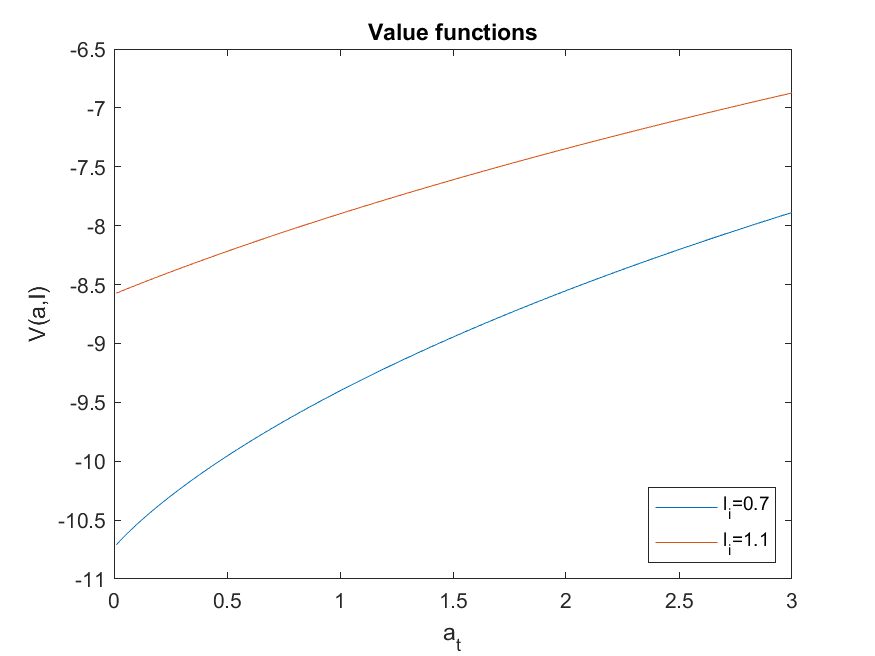
\includegraphics[scale=.75]{figure1.png}
				\end{center}
			
			\item The policy functions, ${a'(a,l_i)}$ are displayed below. There does appear to be a ${\overline{a}\approx 2.175}$ such that ${\forall a\geq\overline{a},a'(a,l_2)<a}$, which is indicated on the chart. The existence of this value and the fact that ${a'(a,l_1)<a}$ for all $a$ suggest that the long-run value of $a_t$ never exceeds $\overline{a}$.
				\begin{center}
					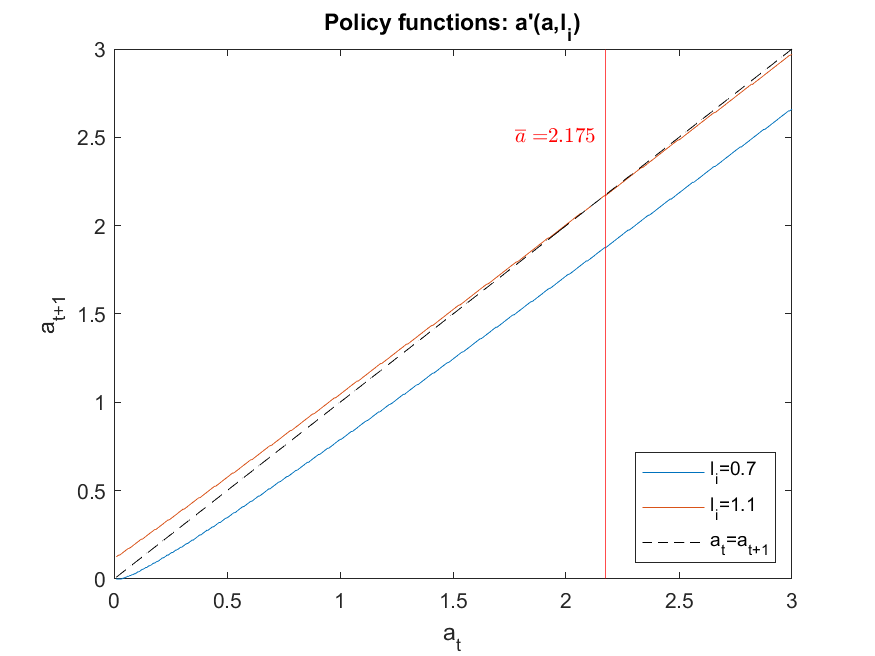
\includegraphics[scale=.75]{figure2.png}
				\end{center}
			
		\end{enumerate}
	
	
	\item The chart below displays the marginal probability mass function for $a_t$, along with its mean, which is ${\approx 1.02}$
		\begin{center}
			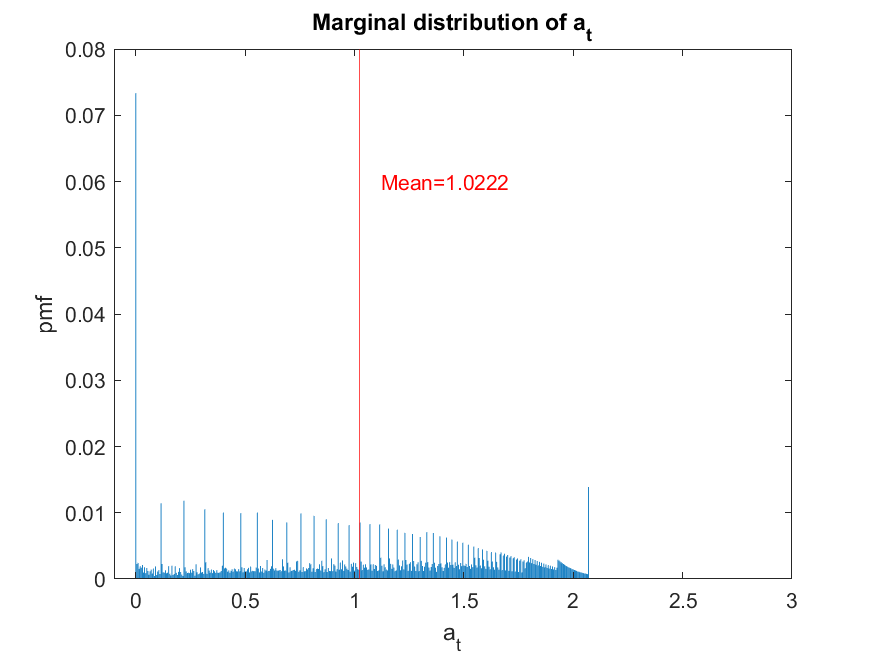
\includegraphics[scale=.75]{figure3.png}
		\end{center}
	
	
\end{enumerate}

%%%________________________________________________________________%%%


\end{document}



%%% RIP!!!!



		
		From this condition, we can derive each of the following conditions:
		\begin{align*}
			\beta^t\frac{(1-\delta)^t}{c_t^1(s_1)} 		&= \lambda^1q_t^0(s^1)	\\
			\beta^t\frac{1-(1-\delta)^t}{c_t^1(s_2)}  	&= \lambda^1q_t^0(s^2)	\\
			\beta^t\frac{(1-\delta)^t}{c_t^2(s_1)}  	&= \lambda^2q_t^0(s^1)	\\
			\beta^t\frac{1-(1-\delta)^t}{c_t^2(s_2)}  	&= \lambda^2q_t^0(s^2)
		\end{align*}
		Combining each consumer's FOC from each states allows us to find a relation that doesn't include the heterogeneous Lagrangian multiplier:
		\[
			\frac{(1-\delta)^t}{1-(1-\delta)^t}\left(\frac{c_t^i(s_2)}{c_t^i(s_1)}\right) = \frac{q_t^0(s^1)}{q_t^0(s^2)}
		\]
		Which can then be combined across consumers to eliminate each state's proability mass:
		\[
			\left(\frac{c_t^2(s_1)}{c_t^1(s_1)}\right)\left(\frac{c_t^1(s_2)}{c_t^2(s_2)}\right) = 1
		\]





